% Options for packages loaded elsewhere
\PassOptionsToPackage{unicode}{hyperref}
\PassOptionsToPackage{hyphens}{url}
%
\documentclass[
]{article}
\usepackage{amsmath,amssymb}
\usepackage{lmodern}
\usepackage{iftex}
\ifPDFTeX
  \usepackage[T1]{fontenc}
  \usepackage[utf8]{inputenc}
  \usepackage{textcomp} % provide euro and other symbols
\else % if luatex or xetex
  \usepackage{unicode-math}
  \defaultfontfeatures{Scale=MatchLowercase}
  \defaultfontfeatures[\rmfamily]{Ligatures=TeX,Scale=1}
\fi
% Use upquote if available, for straight quotes in verbatim environments
\IfFileExists{upquote.sty}{\usepackage{upquote}}{}
\IfFileExists{microtype.sty}{% use microtype if available
  \usepackage[]{microtype}
  \UseMicrotypeSet[protrusion]{basicmath} % disable protrusion for tt fonts
}{}
\makeatletter
\@ifundefined{KOMAClassName}{% if non-KOMA class
  \IfFileExists{parskip.sty}{%
    \usepackage{parskip}
  }{% else
    \setlength{\parindent}{0pt}
    \setlength{\parskip}{6pt plus 2pt minus 1pt}}
}{% if KOMA class
  \KOMAoptions{parskip=half}}
\makeatother
\usepackage{xcolor}
\usepackage[margin=1in]{geometry}
\usepackage{color}
\usepackage{fancyvrb}
\newcommand{\VerbBar}{|}
\newcommand{\VERB}{\Verb[commandchars=\\\{\}]}
\DefineVerbatimEnvironment{Highlighting}{Verbatim}{commandchars=\\\{\}}
% Add ',fontsize=\small' for more characters per line
\usepackage{framed}
\definecolor{shadecolor}{RGB}{248,248,248}
\newenvironment{Shaded}{\begin{snugshade}}{\end{snugshade}}
\newcommand{\AlertTok}[1]{\textcolor[rgb]{0.94,0.16,0.16}{#1}}
\newcommand{\AnnotationTok}[1]{\textcolor[rgb]{0.56,0.35,0.01}{\textbf{\textit{#1}}}}
\newcommand{\AttributeTok}[1]{\textcolor[rgb]{0.77,0.63,0.00}{#1}}
\newcommand{\BaseNTok}[1]{\textcolor[rgb]{0.00,0.00,0.81}{#1}}
\newcommand{\BuiltInTok}[1]{#1}
\newcommand{\CharTok}[1]{\textcolor[rgb]{0.31,0.60,0.02}{#1}}
\newcommand{\CommentTok}[1]{\textcolor[rgb]{0.56,0.35,0.01}{\textit{#1}}}
\newcommand{\CommentVarTok}[1]{\textcolor[rgb]{0.56,0.35,0.01}{\textbf{\textit{#1}}}}
\newcommand{\ConstantTok}[1]{\textcolor[rgb]{0.00,0.00,0.00}{#1}}
\newcommand{\ControlFlowTok}[1]{\textcolor[rgb]{0.13,0.29,0.53}{\textbf{#1}}}
\newcommand{\DataTypeTok}[1]{\textcolor[rgb]{0.13,0.29,0.53}{#1}}
\newcommand{\DecValTok}[1]{\textcolor[rgb]{0.00,0.00,0.81}{#1}}
\newcommand{\DocumentationTok}[1]{\textcolor[rgb]{0.56,0.35,0.01}{\textbf{\textit{#1}}}}
\newcommand{\ErrorTok}[1]{\textcolor[rgb]{0.64,0.00,0.00}{\textbf{#1}}}
\newcommand{\ExtensionTok}[1]{#1}
\newcommand{\FloatTok}[1]{\textcolor[rgb]{0.00,0.00,0.81}{#1}}
\newcommand{\FunctionTok}[1]{\textcolor[rgb]{0.00,0.00,0.00}{#1}}
\newcommand{\ImportTok}[1]{#1}
\newcommand{\InformationTok}[1]{\textcolor[rgb]{0.56,0.35,0.01}{\textbf{\textit{#1}}}}
\newcommand{\KeywordTok}[1]{\textcolor[rgb]{0.13,0.29,0.53}{\textbf{#1}}}
\newcommand{\NormalTok}[1]{#1}
\newcommand{\OperatorTok}[1]{\textcolor[rgb]{0.81,0.36,0.00}{\textbf{#1}}}
\newcommand{\OtherTok}[1]{\textcolor[rgb]{0.56,0.35,0.01}{#1}}
\newcommand{\PreprocessorTok}[1]{\textcolor[rgb]{0.56,0.35,0.01}{\textit{#1}}}
\newcommand{\RegionMarkerTok}[1]{#1}
\newcommand{\SpecialCharTok}[1]{\textcolor[rgb]{0.00,0.00,0.00}{#1}}
\newcommand{\SpecialStringTok}[1]{\textcolor[rgb]{0.31,0.60,0.02}{#1}}
\newcommand{\StringTok}[1]{\textcolor[rgb]{0.31,0.60,0.02}{#1}}
\newcommand{\VariableTok}[1]{\textcolor[rgb]{0.00,0.00,0.00}{#1}}
\newcommand{\VerbatimStringTok}[1]{\textcolor[rgb]{0.31,0.60,0.02}{#1}}
\newcommand{\WarningTok}[1]{\textcolor[rgb]{0.56,0.35,0.01}{\textbf{\textit{#1}}}}
\usepackage{graphicx}
\makeatletter
\def\maxwidth{\ifdim\Gin@nat@width>\linewidth\linewidth\else\Gin@nat@width\fi}
\def\maxheight{\ifdim\Gin@nat@height>\textheight\textheight\else\Gin@nat@height\fi}
\makeatother
% Scale images if necessary, so that they will not overflow the page
% margins by default, and it is still possible to overwrite the defaults
% using explicit options in \includegraphics[width, height, ...]{}
\setkeys{Gin}{width=\maxwidth,height=\maxheight,keepaspectratio}
% Set default figure placement to htbp
\makeatletter
\def\fps@figure{htbp}
\makeatother
\setlength{\emergencystretch}{3em} % prevent overfull lines
\providecommand{\tightlist}{%
  \setlength{\itemsep}{0pt}\setlength{\parskip}{0pt}}
\setcounter{secnumdepth}{-\maxdimen} % remove section numbering
\ifLuaTeX
  \usepackage{selnolig}  % disable illegal ligatures
\fi
\IfFileExists{bookmark.sty}{\usepackage{bookmark}}{\usepackage{hyperref}}
\IfFileExists{xurl.sty}{\usepackage{xurl}}{} % add URL line breaks if available
\urlstyle{same} % disable monospaced font for URLs
\hypersetup{
  pdftitle={HW1-Trinath Sai Subhash Reddy-Pittala},
  pdfauthor={Subhash},
  hidelinks,
  pdfcreator={LaTeX via pandoc}}

\title{HW1-Trinath Sai Subhash Reddy-Pittala}
\author{Subhash}
\date{2023-03-05}

\begin{document}
\maketitle

\begin{Shaded}
\begin{Highlighting}[]
\FunctionTok{library}\NormalTok{(formatR)}
\FunctionTok{library}\NormalTok{(tidyverse)}
\end{Highlighting}
\end{Shaded}

\begin{verbatim}
## -- Attaching packages --------------------------------------- tidyverse 1.3.2 --
## v ggplot2 3.4.0      v purrr   1.0.1 
## v tibble  3.1.8      v dplyr   1.0.10
## v tidyr   1.3.0      v stringr 1.5.0 
## v readr   2.1.3      v forcats 0.5.2 
## -- Conflicts ------------------------------------------ tidyverse_conflicts() --
## x dplyr::filter() masks stats::filter()
## x dplyr::lag()    masks stats::lag()
\end{verbatim}

\begin{Shaded}
\begin{Highlighting}[]
\FunctionTok{library}\NormalTok{(GGally)}
\end{Highlighting}
\end{Shaded}

\begin{verbatim}
## Registered S3 method overwritten by 'GGally':
##   method from   
##   +.gg   ggplot2
\end{verbatim}

\begin{Shaded}
\begin{Highlighting}[]
\FunctionTok{library}\NormalTok{(ggfortify)}
\FunctionTok{library}\NormalTok{(nycflights13)}
\FunctionTok{library}\NormalTok{(modelr)}
\FunctionTok{library}\NormalTok{(magick)}
\end{Highlighting}
\end{Shaded}

\begin{verbatim}
## Linking to ImageMagick 6.9.12.3
## Enabled features: cairo, fontconfig, freetype, heic, lcms, pango, raw, rsvg, webp
## Disabled features: fftw, ghostscript, x11
\end{verbatim}

\begin{Shaded}
\begin{Highlighting}[]
\FunctionTok{library}\NormalTok{(haven)}
\FunctionTok{library}\NormalTok{(dplyr)}
\FunctionTok{library}\NormalTok{(ISLR)}
\FunctionTok{library}\NormalTok{(lubridate)}
\end{Highlighting}
\end{Shaded}

\begin{verbatim}
## 
## Attaching package: 'lubridate'
## 
## The following objects are masked from 'package:base':
## 
##     date, intersect, setdiff, union
\end{verbatim}

\begin{Shaded}
\begin{Highlighting}[]
\FunctionTok{library}\NormalTok{(ggplot2)}
\NormalTok{knitr}\SpecialCharTok{::}\NormalTok{opts\_chunk}\SpecialCharTok{$}\FunctionTok{set}\NormalTok{(}\AttributeTok{width =} \DecValTok{60}\NormalTok{, }\AttributeTok{warning =} \ConstantTok{FALSE}\NormalTok{, }\AttributeTok{message =} \ConstantTok{FALSE}\NormalTok{, }\AttributeTok{tidy.opts=}\FunctionTok{list}\NormalTok{(}\AttributeTok{width.cutoff=}\DecValTok{60}\NormalTok{),}\AttributeTok{tidy=}\ConstantTok{TRUE}\NormalTok{, }\AttributeTok{echo =} \ConstantTok{TRUE}\NormalTok{)}
\CommentTok{\#knitr::opts\_chunk$set(echo = TRUE)}
\end{Highlighting}
\end{Shaded}

\hypertarget{r-working-environment}{%
\section{R Working Environment}\label{r-working-environment}}

Please load all the packages used in the following R chunk before the
function sessionInfo(). This is done using the library() function. e.g.,
library(tidyverse)

\begin{Shaded}
\begin{Highlighting}[]
\FunctionTok{sessionInfo}\NormalTok{()}
\end{Highlighting}
\end{Shaded}

\begin{verbatim}
## R version 4.2.2 (2022-10-31)
## Platform: aarch64-apple-darwin20 (64-bit)
## Running under: macOS Ventura 13.2.1
## 
## Matrix products: default
## BLAS:   /Library/Frameworks/R.framework/Versions/4.2-arm64/Resources/lib/libRblas.0.dylib
## LAPACK: /Library/Frameworks/R.framework/Versions/4.2-arm64/Resources/lib/libRlapack.dylib
## 
## locale:
## [1] en_US.UTF-8/en_US.UTF-8/en_US.UTF-8/C/en_US.UTF-8/en_US.UTF-8
## 
## attached base packages:
## [1] stats     graphics  grDevices utils     datasets  methods   base     
## 
## other attached packages:
##  [1] lubridate_1.9.1    ISLR_1.4           haven_2.5.1        magick_2.7.3      
##  [5] modelr_0.1.10      nycflights13_1.0.2 ggfortify_0.4.15   GGally_2.1.2      
##  [9] forcats_0.5.2      stringr_1.5.0      dplyr_1.0.10       purrr_1.0.1       
## [13] readr_2.1.3        tidyr_1.3.0        tibble_3.1.8       ggplot2_3.4.0     
## [17] tidyverse_1.3.2    formatR_1.14      
## 
## loaded via a namespace (and not attached):
##  [1] Rcpp_1.0.10         assertthat_0.2.1    digest_0.6.31      
##  [4] utf8_1.2.2          R6_2.5.1            cellranger_1.1.0   
##  [7] plyr_1.8.8          backports_1.4.1     reprex_2.0.2       
## [10] evaluate_0.20       httr_1.4.4          pillar_1.8.1       
## [13] rlang_1.0.6         googlesheets4_1.0.1 readxl_1.4.1       
## [16] rstudioapi_0.14     rmarkdown_2.20      googledrive_2.0.0  
## [19] munsell_0.5.0       broom_1.0.3         compiler_4.2.2     
## [22] xfun_0.36           pkgconfig_2.0.3     htmltools_0.5.4    
## [25] tidyselect_1.2.0    gridExtra_2.3       reshape_0.8.9      
## [28] fansi_1.0.4         crayon_1.5.2        tzdb_0.3.0         
## [31] dbplyr_2.3.0        withr_2.5.0         grid_4.2.2         
## [34] jsonlite_1.8.4      gtable_0.3.1        lifecycle_1.0.3    
## [37] DBI_1.1.3           magrittr_2.0.3      scales_1.2.1       
## [40] cli_3.6.0           stringi_1.7.12      fs_1.6.0           
## [43] xml2_1.3.3          ellipsis_0.3.2      generics_0.1.3     
## [46] vctrs_0.5.2         RColorBrewer_1.1-3  tools_4.2.2        
## [49] glue_1.6.2          hms_1.1.2           fastmap_1.1.0      
## [52] yaml_2.3.7          timechange_0.2.0    colorspace_2.1-0   
## [55] gargle_1.2.1        rvest_1.0.3         knitr_1.42
\end{verbatim}

\hypertarget{working-with-data}{%
\section{Working with data}\label{working-with-data}}

\begin{enumerate}
\def\labelenumi{\arabic{enumi}.}
\tightlist
\item
  The data set rnf6080.dat records hourly rainfall at a certain location
  in Canada, every day from 1960 to 1980.
\end{enumerate}

\begin{enumerate}
\def\labelenumi{\alph{enumi}.}
\tightlist
\item
  Load the data set into R and make it a data frame called rain.df. What
  command did you use?
\end{enumerate}

\begin{Shaded}
\begin{Highlighting}[]
\NormalTok{rain.df }\OtherTok{\textless{}{-}} \FunctionTok{read.table}\NormalTok{(}\StringTok{"rnf6080.dat"}\NormalTok{)}
\FunctionTok{head}\NormalTok{(rain.df)}
\end{Highlighting}
\end{Shaded}

\begin{verbatim}
##   V1 V2 V3 V4 V5 V6 V7 V8 V9 V10 V11 V12 V13 V14 V15 V16 V17 V18 V19 V20 V21
## 1 60  4  1  0  0  0  0  0  0   0   0   0   0   0   0   0   0   0   0   0   0
## 2 60  4  2  0  0  0  0  0  0   0   0   0   0   0   0   0   0   0   0   0   0
## 3 60  4  3  0  0  0  0  0  0   0   0   0   0   0   0   0   0   0   0   0   0
## 4 60  4  4  0  0  0  0  0  0   0   0   0   0   0   0   0   0   0   0   0   0
## 5 60  4  5  0  0  0  0  0  0   0   0   0   0   0   0   0   0   0   0   0   0
## 6 60  4  6  0  0  0  0  0  0   0   0   0   0   0   0   0   0   0   0   0   0
##   V22 V23 V24 V25 V26 V27
## 1   0   0   0   0   0   0
## 2   0   0   0   0   0   0
## 3   0   0   0   0   0   0
## 4   0   0   0   0   0   0
## 5   0   0   0   0   0   0
## 6   0   0   0   0   0   0
\end{verbatim}

\begin{enumerate}
\def\labelenumi{\alph{enumi}.}
\setcounter{enumi}{1}
\tightlist
\item
  How many rows and columns does rain.df have? How do you know? (If
  there are not 5070 rows and 27 columns, you did something wrong in the
  first part of the problem.)
\end{enumerate}

\begin{Shaded}
\begin{Highlighting}[]
\FunctionTok{nrow}\NormalTok{(rain.df)}
\end{Highlighting}
\end{Shaded}

\begin{verbatim}
## [1] 5070
\end{verbatim}

\begin{Shaded}
\begin{Highlighting}[]
\FunctionTok{ncol}\NormalTok{(rain.df)}
\end{Highlighting}
\end{Shaded}

\begin{verbatim}
## [1] 27
\end{verbatim}

\begin{enumerate}
\def\labelenumi{\alph{enumi}.}
\setcounter{enumi}{2}
\tightlist
\item
  What command would you use to get the names of the columns of rain.df?
  What are those names?
\end{enumerate}

\begin{Shaded}
\begin{Highlighting}[]
\FunctionTok{colnames}\NormalTok{(rain.df)}
\end{Highlighting}
\end{Shaded}

\begin{verbatim}
##  [1] "V1"  "V2"  "V3"  "V4"  "V5"  "V6"  "V7"  "V8"  "V9"  "V10" "V11" "V12"
## [13] "V13" "V14" "V15" "V16" "V17" "V18" "V19" "V20" "V21" "V22" "V23" "V24"
## [25] "V25" "V26" "V27"
\end{verbatim}

\begin{enumerate}
\def\labelenumi{\alph{enumi}.}
\setcounter{enumi}{3}
\tightlist
\item
  What command would you use to get the value at row 2, column 4? What
  is the value?
\end{enumerate}

\begin{Shaded}
\begin{Highlighting}[]
\NormalTok{rain.df[}\DecValTok{2}\NormalTok{, }\DecValTok{4}\NormalTok{]}
\end{Highlighting}
\end{Shaded}

\begin{verbatim}
## [1] 0
\end{verbatim}

\begin{enumerate}
\def\labelenumi{\alph{enumi}.}
\setcounter{enumi}{4}
\tightlist
\item
  What command would you use to display the whole second row? What is
  the content of that row?
\end{enumerate}

\begin{Shaded}
\begin{Highlighting}[]
\NormalTok{rain.df[}\DecValTok{2}\NormalTok{, ]}
\end{Highlighting}
\end{Shaded}

\begin{verbatim}
##   V1 V2 V3 V4 V5 V6 V7 V8 V9 V10 V11 V12 V13 V14 V15 V16 V17 V18 V19 V20 V21
## 2 60  4  2  0  0  0  0  0  0   0   0   0   0   0   0   0   0   0   0   0   0
##   V22 V23 V24 V25 V26 V27
## 2   0   0   0   0   0   0
\end{verbatim}

\begin{enumerate}
\def\labelenumi{\alph{enumi}.}
\setcounter{enumi}{5}
\tightlist
\item
  What does the following command do?
\end{enumerate}

\begin{Shaded}
\begin{Highlighting}[]
\FunctionTok{names}\NormalTok{(rain.df) }\OtherTok{\textless{}{-}} \FunctionTok{c}\NormalTok{(}\StringTok{"year"}\NormalTok{, }\StringTok{"month"}\NormalTok{, }\StringTok{"day"}\NormalTok{, }\FunctionTok{seq}\NormalTok{(}\DecValTok{0}\NormalTok{, }\DecValTok{23}\NormalTok{))}
\end{Highlighting}
\end{Shaded}

It renames column names to Year Month Day and 0 to 23 for the rest.

\begin{enumerate}
\def\labelenumi{\alph{enumi}.}
\setcounter{enumi}{6}
\tightlist
\item
  Create a new column called daily, which is the sum of the 24 hourly
  columns.
\end{enumerate}

\begin{Shaded}
\begin{Highlighting}[]
\NormalTok{rain.df }\OtherTok{\textless{}{-}} \FunctionTok{mutate}\NormalTok{(rain.df, }\AttributeTok{daily =} \StringTok{\textasciigrave{}}\AttributeTok{0}\StringTok{\textasciigrave{}} \SpecialCharTok{+} \StringTok{\textasciigrave{}}\AttributeTok{1}\StringTok{\textasciigrave{}} \SpecialCharTok{+} \StringTok{\textasciigrave{}}\AttributeTok{2}\StringTok{\textasciigrave{}} \SpecialCharTok{+} \StringTok{\textasciigrave{}}\AttributeTok{3}\StringTok{\textasciigrave{}} \SpecialCharTok{+} \StringTok{\textasciigrave{}}\AttributeTok{4}\StringTok{\textasciigrave{}} \SpecialCharTok{+}
    \StringTok{\textasciigrave{}}\AttributeTok{5}\StringTok{\textasciigrave{}} \SpecialCharTok{+} \StringTok{\textasciigrave{}}\AttributeTok{6}\StringTok{\textasciigrave{}} \SpecialCharTok{+} \StringTok{\textasciigrave{}}\AttributeTok{7}\StringTok{\textasciigrave{}} \SpecialCharTok{+} \StringTok{\textasciigrave{}}\AttributeTok{8}\StringTok{\textasciigrave{}} \SpecialCharTok{+} \StringTok{\textasciigrave{}}\AttributeTok{9}\StringTok{\textasciigrave{}} \SpecialCharTok{+} \StringTok{\textasciigrave{}}\AttributeTok{10}\StringTok{\textasciigrave{}} \SpecialCharTok{+} \StringTok{\textasciigrave{}}\AttributeTok{11}\StringTok{\textasciigrave{}} \SpecialCharTok{+} \StringTok{\textasciigrave{}}\AttributeTok{12}\StringTok{\textasciigrave{}} \SpecialCharTok{+} \StringTok{\textasciigrave{}}\AttributeTok{13}\StringTok{\textasciigrave{}} \SpecialCharTok{+}
    \StringTok{\textasciigrave{}}\AttributeTok{14}\StringTok{\textasciigrave{}} \SpecialCharTok{+} \StringTok{\textasciigrave{}}\AttributeTok{15}\StringTok{\textasciigrave{}} \SpecialCharTok{+} \StringTok{\textasciigrave{}}\AttributeTok{16}\StringTok{\textasciigrave{}} \SpecialCharTok{+} \StringTok{\textasciigrave{}}\AttributeTok{17}\StringTok{\textasciigrave{}} \SpecialCharTok{+} \StringTok{\textasciigrave{}}\AttributeTok{18}\StringTok{\textasciigrave{}} \SpecialCharTok{+} \StringTok{\textasciigrave{}}\AttributeTok{19}\StringTok{\textasciigrave{}} \SpecialCharTok{+} \StringTok{\textasciigrave{}}\AttributeTok{20}\StringTok{\textasciigrave{}} \SpecialCharTok{+} \StringTok{\textasciigrave{}}\AttributeTok{21}\StringTok{\textasciigrave{}} \SpecialCharTok{+} \StringTok{\textasciigrave{}}\AttributeTok{22}\StringTok{\textasciigrave{}} \SpecialCharTok{+}
    \StringTok{\textasciigrave{}}\AttributeTok{23}\StringTok{\textasciigrave{}}\NormalTok{)}
\end{Highlighting}
\end{Shaded}

\begin{enumerate}
\def\labelenumi{\alph{enumi}.}
\setcounter{enumi}{7}
\tightlist
\item
  Give the command you would use to create a histogram of the daily
  rainfall amounts. Please make sure to attach your figures in your .pdf
  report.
\end{enumerate}

\begin{Shaded}
\begin{Highlighting}[]
\FunctionTok{hist}\NormalTok{(rain.df}\SpecialCharTok{$}\NormalTok{daily)}
\end{Highlighting}
\end{Shaded}

\includegraphics{HW1-Trinath-Sai-Subhash-Reddy-Pittala_files/figure-latex/unnamed-chunk-9-1.pdf}

\begin{enumerate}
\def\labelenumi{\roman{enumi}.}
\tightlist
\item
  Explain why that histogram above cannot possibly be right.
\end{enumerate}

It is not correct because rainfall cant be negative. This is occuring
due to NA being replaced as -999 in data.

\begin{enumerate}
\def\labelenumi{\alph{enumi}.}
\setcounter{enumi}{9}
\tightlist
\item
  Give the command you would use to fix the data frame.
\end{enumerate}

\begin{Shaded}
\begin{Highlighting}[]
\NormalTok{rain.df[rain.df }\SpecialCharTok{==} \SpecialCharTok{{-}}\DecValTok{999}\NormalTok{] }\OtherTok{\textless{}{-}} \ConstantTok{NA}
\NormalTok{rain.df}\SpecialCharTok{$}\NormalTok{daily }\OtherTok{\textless{}{-}} \FunctionTok{c}\NormalTok{(}\FunctionTok{rowSums}\NormalTok{(rain.df[, }\DecValTok{4}\SpecialCharTok{:}\DecValTok{27}\NormalTok{], }\AttributeTok{na.rm =} \ConstantTok{TRUE}\NormalTok{))}
\end{Highlighting}
\end{Shaded}

\begin{enumerate}
\def\labelenumi{\alph{enumi}.}
\setcounter{enumi}{10}
\tightlist
\item
  Create a corrected histogram and again include it as part of your
  submitted report. Explain why it is more reasonable than the previous
  histogram.
\end{enumerate}

\begin{Shaded}
\begin{Highlighting}[]
\FunctionTok{hist}\NormalTok{(rain.df}\SpecialCharTok{$}\NormalTok{daily)}
\end{Highlighting}
\end{Shaded}

\includegraphics{HW1-Trinath-Sai-Subhash-Reddy-Pittala_files/figure-latex/unnamed-chunk-11-1.pdf}

This is more reasonable graph because it is showing the right skewed
normal distribution without any obvious abnormalities like negative
rainfall.

\hypertarget{data-types}{%
\section{Data types}\label{data-types}}

\begin{enumerate}
\def\labelenumi{\arabic{enumi}.}
\setcounter{enumi}{1}
\tightlist
\item
  Make sure your answers to different parts of this problem are
  compatible with each other.
\end{enumerate}

\begin{enumerate}
\def\labelenumi{\alph{enumi}.}
\tightlist
\item
  For each of the following commands, either explain why they should be
  errors, or explain the non- erroneous result.
\end{enumerate}

\begin{Shaded}
\begin{Highlighting}[]
\NormalTok{x }\OtherTok{\textless{}{-}} \FunctionTok{c}\NormalTok{(}\StringTok{"5"}\NormalTok{, }\StringTok{"12"}\NormalTok{, }\StringTok{"7"}\NormalTok{)}
\FunctionTok{max}\NormalTok{(x)}
\FunctionTok{sort}\NormalTok{(x)}
\FunctionTok{sum}\NormalTok{(x)}
\end{Highlighting}
\end{Shaded}

There are errors, because we are intializing the numbers to be character
strings.

max(x) finds max in numeric vector. On character vector it returns
character with highest index.

sort(x) sort in lexograpical order in character vector. So result would
be \{``12'', ``5'', ``7''\}

sum(x) will throw error because of invalid type of argument.

\begin{enumerate}
\def\labelenumi{\alph{enumi}.}
\setcounter{enumi}{1}
\tightlist
\item
  For the next two commands, either explain their results, or why they
  should produce errors.
\end{enumerate}

\begin{Shaded}
\begin{Highlighting}[]
\NormalTok{y }\OtherTok{\textless{}{-}} \FunctionTok{c}\NormalTok{(}\StringTok{"5"}\NormalTok{, }\DecValTok{7}\NormalTok{, }\DecValTok{12}\NormalTok{)}
\NormalTok{y[}\DecValTok{2}\NormalTok{] }\SpecialCharTok{+}\NormalTok{ y[}\DecValTok{3}\NormalTok{]}
\end{Highlighting}
\end{Shaded}

We are creating a vector y with three elements, where the first element
is a character string, and rest numeric.

y{[}2{]} + y{[}3{]} will throw an error since y{[}1{]} is character
string.

\begin{enumerate}
\def\labelenumi{\alph{enumi}.}
\setcounter{enumi}{2}
\tightlist
\item
  For the next two commands, either explain their results, or why they
  should produce errors.
\end{enumerate}

\begin{Shaded}
\begin{Highlighting}[]
\NormalTok{z }\OtherTok{\textless{}{-}} \FunctionTok{data.frame}\NormalTok{(}\AttributeTok{z1 =} \StringTok{"5"}\NormalTok{, }\AttributeTok{z2 =} \DecValTok{7}\NormalTok{, }\AttributeTok{z3 =} \DecValTok{12}\NormalTok{)}
\NormalTok{z[}\DecValTok{1}\NormalTok{, }\DecValTok{2}\NormalTok{] }\SpecialCharTok{+}\NormalTok{ z[}\DecValTok{1}\NormalTok{, }\DecValTok{3}\NormalTok{]}
\end{Highlighting}
\end{Shaded}

\begin{verbatim}
## [1] 19
\end{verbatim}

We are creating a data frame z with three columns and one row. The first
column is a character string, and rest numeric.

z{[}1,2{]} + z{[}1,3{]} result 19, unlike above case in this case each
vector is taken column wise so errors pop up.

\hypertarget{linear-algebra}{%
\section{Linear algebra}\label{linear-algebra}}

\begin{enumerate}
\def\labelenumi{\arabic{enumi}.}
\setcounter{enumi}{2}
\tightlist
\item
  Consider the linear system AX = b. Please answer the following
  questions
\end{enumerate}

\begin{enumerate}
\def\labelenumi{\alph{enumi}.}
\tightlist
\item
  Write an R function called my\_solver() such that given inputs A and
  b, the function my\_solver() returns the solution of the linear system
\end{enumerate}

\begin{Shaded}
\begin{Highlighting}[]
\NormalTok{my\_solver }\OtherTok{\textless{}{-}} \ControlFlowTok{function}\NormalTok{(A, b) \{}
\NormalTok{    X }\OtherTok{\textless{}{-}} \FunctionTok{solve}\NormalTok{(A, b)}
    \FunctionTok{return}\NormalTok{(X)}
\NormalTok{\}}
\end{Highlighting}
\end{Shaded}

\begin{enumerate}
\def\labelenumi{\alph{enumi}.}
\setcounter{enumi}{1}
\tightlist
\item
  Run the following code to get A and b.
\end{enumerate}

\begin{Shaded}
\begin{Highlighting}[]
\NormalTok{n }\OtherTok{\textless{}{-}} \DecValTok{100}
\FunctionTok{set.seed}\NormalTok{(}\DecValTok{123}\NormalTok{)}
\NormalTok{A }\OtherTok{\textless{}{-}} \FunctionTok{rWishart}\NormalTok{(}\DecValTok{1}\NormalTok{, }\DecValTok{150}\NormalTok{, }\FunctionTok{diag}\NormalTok{(n))[, , }\DecValTok{1}\NormalTok{]}
\NormalTok{b }\OtherTok{\textless{}{-}} \FunctionTok{rnorm}\NormalTok{(n, }\DecValTok{1}\NormalTok{)}
\NormalTok{X }\OtherTok{\textless{}{-}} \FunctionTok{my\_solver}\NormalTok{(A, b)}
\end{Highlighting}
\end{Shaded}

Verifying

\begin{Shaded}
\begin{Highlighting}[]
\NormalTok{AX }\OtherTok{=}\NormalTok{ A }\SpecialCharTok{\%*\%}\NormalTok{ X}
\NormalTok{AX }\OtherTok{\textless{}{-}} \FunctionTok{as.numeric}\NormalTok{(AX)}
\FunctionTok{all.equal}\NormalTok{(AX, b, }\AttributeTok{tolerance =} \FloatTok{1e{-}06}\NormalTok{)}
\end{Highlighting}
\end{Shaded}

\begin{verbatim}
## [1] TRUE
\end{verbatim}

\hypertarget{working-with-ggplot2}{%
\section{Working with ggplot2}\label{working-with-ggplot2}}

\begin{enumerate}
\def\labelenumi{\arabic{enumi}.}
\setcounter{enumi}{3}
\tightlist
\item
  EPA monitors Air Quality data across the entire U.S. The file
  ``AQSdata.csv'' contains daily PM 2.5 concentrations and other
  information. Please make the following questions using the ggplot()
  function for plotting. In addition make sure that all the x-axis and
  y-axis labels have 14 font size.
\end{enumerate}

\begin{enumerate}
\def\labelenumi{\alph{enumi}.}
\item
  Read the data file ``AQSdata.csv'' into R.
\item
  Generate density plots of PM2.5 concentrations grouped by County in
  one single panel, where each density should have its own color. What
  do you find from the figure?
\end{enumerate}

\begin{Shaded}
\begin{Highlighting}[]
\FunctionTok{ggplot}\NormalTok{(AQSdata, }\FunctionTok{aes}\NormalTok{(}\AttributeTok{x =}\NormalTok{ PM2}\FloatTok{.5}\NormalTok{, }\AttributeTok{fill =}\NormalTok{ COUNTY)) }\SpecialCharTok{+} \FunctionTok{geom\_density}\NormalTok{(}\AttributeTok{alpha =} \FloatTok{0.5}\NormalTok{) }\SpecialCharTok{+}
    \FunctionTok{theme}\NormalTok{(}\AttributeTok{axis.title.x =} \FunctionTok{element\_text}\NormalTok{(}\AttributeTok{size =} \DecValTok{14}\NormalTok{), }\AttributeTok{axis.title.y =} \FunctionTok{element\_text}\NormalTok{(}\AttributeTok{size =} \DecValTok{14}\NormalTok{))}
\end{Highlighting}
\end{Shaded}

\includegraphics{HW1-Trinath-Sai-Subhash-Reddy-Pittala_files/figure-latex/unnamed-chunk-19-1.pdf}

\begin{enumerate}
\def\labelenumi{\alph{enumi}.}
\setcounter{enumi}{2}
\tightlist
\item
  Plot histograms of PM2.5 concentrations across different counties with
  one panel for one histogram.
\end{enumerate}

\begin{Shaded}
\begin{Highlighting}[]
\FunctionTok{ggplot}\NormalTok{(AQSdata, }\FunctionTok{aes}\NormalTok{(}\AttributeTok{x =}\NormalTok{ PM2}\FloatTok{.5}\NormalTok{, }\AttributeTok{fill =}\NormalTok{ COUNTY)) }\SpecialCharTok{+} \FunctionTok{geom\_histogram}\NormalTok{(}\AttributeTok{alpha =} \FloatTok{0.5}\NormalTok{) }\SpecialCharTok{+}
    \FunctionTok{theme}\NormalTok{(}\AttributeTok{axis.title.x =} \FunctionTok{element\_text}\NormalTok{(}\AttributeTok{size =} \DecValTok{14}\NormalTok{), }\AttributeTok{axis.title.y =} \FunctionTok{element\_text}\NormalTok{(}\AttributeTok{size =} \DecValTok{14}\NormalTok{)) }\SpecialCharTok{+}
    \FunctionTok{facet\_wrap}\NormalTok{(}\SpecialCharTok{\textasciitilde{}}\NormalTok{COUNTY\_CODE, }\AttributeTok{ncol =} \DecValTok{2}\NormalTok{)}
\end{Highlighting}
\end{Shaded}

\includegraphics{HW1-Trinath-Sai-Subhash-Reddy-Pittala_files/figure-latex/unnamed-chunk-20-1.pdf}

\begin{enumerate}
\def\labelenumi{\alph{enumi}.}
\setcounter{enumi}{3}
\tightlist
\item
  Generate boxplots of PM2.5 concentrations by County. What would you
  say about the distributions?
\end{enumerate}

\begin{Shaded}
\begin{Highlighting}[]
\CommentTok{\# Fill = COUNTY for Legend}
\FunctionTok{ggplot}\NormalTok{(AQSdata, }\FunctionTok{aes}\NormalTok{(}\AttributeTok{x =}\NormalTok{ PM2}\FloatTok{.5}\NormalTok{, }\AttributeTok{y =}\NormalTok{ COUNTY)) }\SpecialCharTok{+} \FunctionTok{geom\_boxplot}\NormalTok{() }\SpecialCharTok{+}
    \FunctionTok{theme}\NormalTok{(}\AttributeTok{axis.title.x =} \FunctionTok{element\_text}\NormalTok{(}\AttributeTok{size =} \DecValTok{14}\NormalTok{), }\AttributeTok{axis.title.y =} \FunctionTok{element\_text}\NormalTok{(}\AttributeTok{size =} \DecValTok{14}\NormalTok{))}
\end{Highlighting}
\end{Shaded}

\includegraphics{HW1-Trinath-Sai-Subhash-Reddy-Pittala_files/figure-latex/unnamed-chunk-21-1.pdf}

\begin{enumerate}
\def\labelenumi{\alph{enumi}.}
\setcounter{enumi}{4}
\tightlist
\item
  Reorder the boxplots above by the median value of PM2.5
  concentrations.
\end{enumerate}

\begin{Shaded}
\begin{Highlighting}[]
\NormalTok{aqs\_data\_median }\OtherTok{\textless{}{-}} \FunctionTok{aggregate}\NormalTok{(PM2}\FloatTok{.5} \SpecialCharTok{\textasciitilde{}}\NormalTok{ COUNTY, }\AttributeTok{data =}\NormalTok{ AQSdata,}
\NormalTok{    median)}
\NormalTok{aqs\_data\_median}\SpecialCharTok{$}\NormalTok{County }\OtherTok{\textless{}{-}} \FunctionTok{reorder}\NormalTok{(aqs\_data\_median}\SpecialCharTok{$}\NormalTok{COUNTY, aqs\_data\_median}\SpecialCharTok{$}\NormalTok{PM2}\FloatTok{.5}\NormalTok{)}

\FunctionTok{ggplot}\NormalTok{(AQSdata, }\FunctionTok{aes}\NormalTok{(}\AttributeTok{x =} \FunctionTok{reorder}\NormalTok{(COUNTY, PM2}\FloatTok{.5}\NormalTok{), }\AttributeTok{y =}\NormalTok{ PM2}\FloatTok{.5}\NormalTok{)) }\SpecialCharTok{+}
    \FunctionTok{geom\_boxplot}\NormalTok{() }\SpecialCharTok{+} \FunctionTok{theme}\NormalTok{(}\AttributeTok{axis.title.x =} \FunctionTok{element\_text}\NormalTok{(}\AttributeTok{size =} \DecValTok{14}\NormalTok{),}
    \AttributeTok{axis.title.y =} \FunctionTok{element\_text}\NormalTok{(}\AttributeTok{size =} \DecValTok{14}\NormalTok{)) }\SpecialCharTok{+} \FunctionTok{coord\_flip}\NormalTok{()}
\end{Highlighting}
\end{Shaded}

\includegraphics{HW1-Trinath-Sai-Subhash-Reddy-Pittala_files/figure-latex/unnamed-chunk-22-1.pdf}

\begin{enumerate}
\def\labelenumi{\alph{enumi}.}
\setcounter{enumi}{5}
\tightlist
\item
  Converting the Site ID to a factor and plot the histogram grouped by
  Site ID.
\end{enumerate}

\begin{Shaded}
\begin{Highlighting}[]
\FunctionTok{ggplot}\NormalTok{(AQSdata, }\FunctionTok{aes}\NormalTok{(}\AttributeTok{x =}\NormalTok{ SiteID, }\AttributeTok{color =} \FunctionTok{as.factor}\NormalTok{(SiteID), }\AttributeTok{fill =} \FunctionTok{as.factor}\NormalTok{(SiteID))) }\SpecialCharTok{+}
    \FunctionTok{geom\_histogram}\NormalTok{() }\SpecialCharTok{+} \FunctionTok{theme}\NormalTok{(}\AttributeTok{axis.title.x =} \FunctionTok{element\_text}\NormalTok{(}\AttributeTok{size =} \DecValTok{14}\NormalTok{),}
    \AttributeTok{axis.title.y =} \FunctionTok{element\_text}\NormalTok{(}\AttributeTok{size =} \DecValTok{14}\NormalTok{))}
\end{Highlighting}
\end{Shaded}

\includegraphics{HW1-Trinath-Sai-Subhash-Reddy-Pittala_files/figure-latex/unnamed-chunk-23-1.pdf}

\begin{enumerate}
\def\labelenumi{\alph{enumi}.}
\setcounter{enumi}{6}
\tightlist
\item
  Generate the time series plot for the monitoring Site ID 450190048.
\end{enumerate}

\begin{Shaded}
\begin{Highlighting}[]
\NormalTok{AQSdata\_site }\OtherTok{\textless{}{-}}\NormalTok{ AQSdata[AQSdata}\SpecialCharTok{$}\NormalTok{SiteID }\SpecialCharTok{==} \StringTok{"450190048"}\NormalTok{, ]}
\FunctionTok{ggplot}\NormalTok{(AQSdata\_site, }\FunctionTok{aes}\NormalTok{(}\AttributeTok{x =} \FunctionTok{as.Date}\NormalTok{(Date, }\StringTok{"\%m/\%d/\%y"}\NormalTok{), }\AttributeTok{y =}\NormalTok{ PM2}\FloatTok{.5}\NormalTok{)) }\SpecialCharTok{+}
    \FunctionTok{geom\_line}\NormalTok{() }\SpecialCharTok{+} \FunctionTok{theme}\NormalTok{(}\AttributeTok{axis.title.x =} \FunctionTok{element\_text}\NormalTok{(}\AttributeTok{size =} \DecValTok{14}\NormalTok{),}
    \AttributeTok{axis.title.y =} \FunctionTok{element\_text}\NormalTok{(}\AttributeTok{size =} \DecValTok{14}\NormalTok{)) }\SpecialCharTok{+} \FunctionTok{xlab}\NormalTok{(}\StringTok{"Date"}\NormalTok{)}
\end{Highlighting}
\end{Shaded}

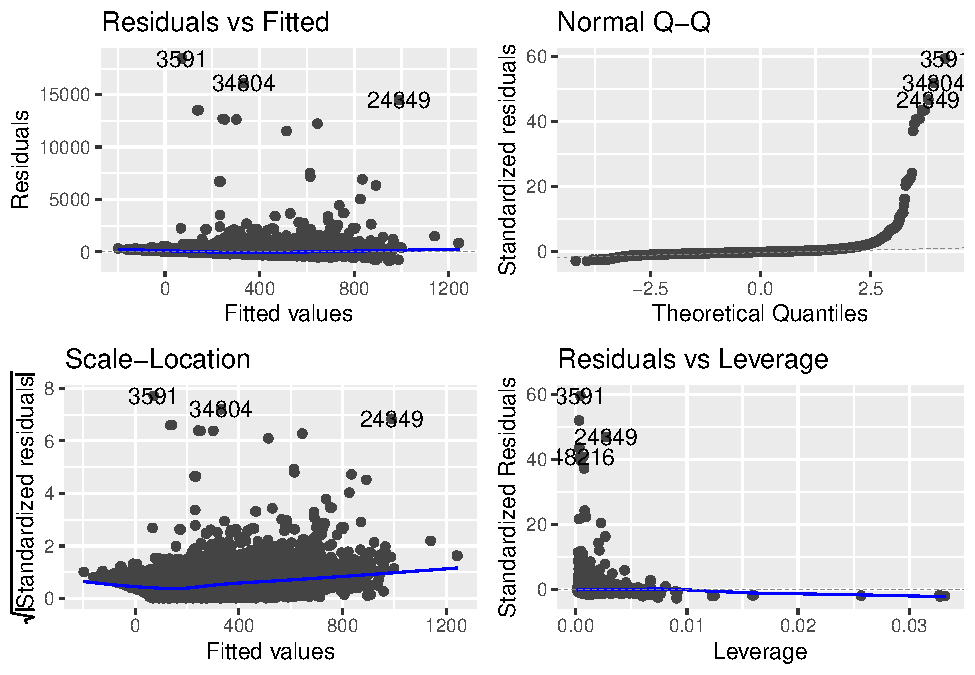
\includegraphics{HW1-Trinath-Sai-Subhash-Reddy-Pittala_files/figure-latex/unnamed-chunk-24-1.pdf}

\begin{enumerate}
\def\labelenumi{\alph{enumi}.}
\setcounter{enumi}{7}
\tightlist
\item
  Plot time series of PM2.5 concentrations for all monitoring sites in
  one panel, where each site has its own color
\end{enumerate}

\begin{Shaded}
\begin{Highlighting}[]
\FunctionTok{ggplot}\NormalTok{(AQSdata, }\FunctionTok{aes}\NormalTok{(}\AttributeTok{x =} \FunctionTok{as.Date}\NormalTok{(Date, }\StringTok{"\%m/\%d/\%y"}\NormalTok{), }\AttributeTok{y =}\NormalTok{ PM2}\FloatTok{.5}\NormalTok{,}
    \AttributeTok{color =}\NormalTok{ SiteID)) }\SpecialCharTok{+} \FunctionTok{geom\_line}\NormalTok{() }\SpecialCharTok{+} \FunctionTok{theme}\NormalTok{(}\AttributeTok{axis.title.x =} \FunctionTok{element\_text}\NormalTok{(}\AttributeTok{size =} \DecValTok{14}\NormalTok{),}
    \AttributeTok{axis.title.y =} \FunctionTok{element\_text}\NormalTok{(}\AttributeTok{size =} \DecValTok{14}\NormalTok{)) }\SpecialCharTok{+} \FunctionTok{xlab}\NormalTok{(}\StringTok{"Date"}\NormalTok{)}
\end{Highlighting}
\end{Shaded}

\includegraphics{HW1-Trinath-Sai-Subhash-Reddy-Pittala_files/figure-latex/unnamed-chunk-25-1.pdf}

\begin{enumerate}
\def\labelenumi{\roman{enumi}.}
\tightlist
\item
  Plot time series of PM2.5 concentrations across all monitoring sites
  in multiple panels, where one panel only has one site, and each row
  only has two panels.
\end{enumerate}

\begin{Shaded}
\begin{Highlighting}[]
\FunctionTok{ggplot}\NormalTok{(AQSdata, }\FunctionTok{aes}\NormalTok{(}\AttributeTok{x =} \FunctionTok{as.Date}\NormalTok{(Date, }\StringTok{"\%m/\%d/\%y"}\NormalTok{), }\AttributeTok{y =}\NormalTok{ PM2}\FloatTok{.5}\NormalTok{,}
    \AttributeTok{color =}\NormalTok{ SiteID)) }\SpecialCharTok{+} \FunctionTok{geom\_line}\NormalTok{() }\SpecialCharTok{+} \FunctionTok{theme}\NormalTok{(}\AttributeTok{text =} \FunctionTok{element\_text}\NormalTok{(}\AttributeTok{size =} \DecValTok{14}\NormalTok{)) }\SpecialCharTok{+}
    \FunctionTok{xlab}\NormalTok{(}\StringTok{"Date"}\NormalTok{) }\SpecialCharTok{+} \FunctionTok{ylab}\NormalTok{(}\StringTok{"PM2.5 Concentration"}\NormalTok{) }\SpecialCharTok{+} \FunctionTok{facet\_wrap}\NormalTok{(}\SpecialCharTok{\textasciitilde{}}\NormalTok{SiteID,}
    \AttributeTok{ncol =} \DecValTok{2}\NormalTok{)}
\end{Highlighting}
\end{Shaded}

\includegraphics{HW1-Trinath-Sai-Subhash-Reddy-Pittala_files/figure-latex/unnamed-chunk-26-1.pdf}

\begin{enumerate}
\def\labelenumi{\alph{enumi}.}
\setcounter{enumi}{9}
\tightlist
\item
  In the time series plot, there seems to be not enough space to hold
  the x-axis labels. One way to avoid this is to rotate the axis labels.
  Please rotate all the time labels 45 degree.
\end{enumerate}

\begin{Shaded}
\begin{Highlighting}[]
\FunctionTok{ggplot}\NormalTok{(AQSdata, }\FunctionTok{aes}\NormalTok{(}\AttributeTok{x =} \FunctionTok{as.Date}\NormalTok{(Date, }\StringTok{"\%m/\%d/\%y"}\NormalTok{), }\AttributeTok{y =}\NormalTok{ PM2}\FloatTok{.5}\NormalTok{,}
    \AttributeTok{color =}\NormalTok{ SiteID)) }\SpecialCharTok{+} \FunctionTok{geom\_line}\NormalTok{() }\SpecialCharTok{+} \FunctionTok{theme}\NormalTok{(}\AttributeTok{text =} \FunctionTok{element\_text}\NormalTok{(}\AttributeTok{size =} \DecValTok{14}\NormalTok{)) }\SpecialCharTok{+}
    \FunctionTok{theme}\NormalTok{(}\AttributeTok{axis.text.x =} \FunctionTok{element\_text}\NormalTok{(}\AttributeTok{angle =} \DecValTok{45}\NormalTok{, }\AttributeTok{hjust =} \DecValTok{1}\NormalTok{)) }\SpecialCharTok{+}
    \FunctionTok{theme}\NormalTok{(}\AttributeTok{axis.text.y =} \FunctionTok{element\_text}\NormalTok{(}\AttributeTok{angle =} \DecValTok{45}\NormalTok{, }\AttributeTok{hjust =} \DecValTok{1}\NormalTok{)) }\SpecialCharTok{+}
    \FunctionTok{xlab}\NormalTok{(}\StringTok{"Date"}\NormalTok{) }\SpecialCharTok{+} \FunctionTok{ylab}\NormalTok{(}\StringTok{"PM2.5 Concentration"}\NormalTok{) }\SpecialCharTok{+} \FunctionTok{facet\_wrap}\NormalTok{(}\SpecialCharTok{\textasciitilde{}}\NormalTok{SiteID,}
    \AttributeTok{ncol =} \DecValTok{2}\NormalTok{)}
\end{Highlighting}
\end{Shaded}

\includegraphics{HW1-Trinath-Sai-Subhash-Reddy-Pittala_files/figure-latex/unnamed-chunk-27-1.pdf}

\hypertarget{working-with-dplyr}{%
\section{Working with dplyr}\label{working-with-dplyr}}

\begin{enumerate}
\def\labelenumi{\arabic{enumi}.}
\setcounter{enumi}{4}
\tightlist
\item
  Continuing working with the above PM 2.5 data.
\end{enumerate}

\begin{enumerate}
\def\labelenumi{\alph{enumi}.}
\tightlist
\item
  Filter all the observations in the county Greenville. How many
  observations are there?
\end{enumerate}

\begin{Shaded}
\begin{Highlighting}[]
\NormalTok{greenville\_data }\OtherTok{\textless{}{-}}\NormalTok{ AQSdata }\SpecialCharTok{\%\textgreater{}\%}
    \FunctionTok{filter}\NormalTok{(COUNTY }\SpecialCharTok{==} \StringTok{"Greenville"}\NormalTok{)}

\FunctionTok{nrow}\NormalTok{(greenville\_data)}
\end{Highlighting}
\end{Shaded}

\begin{verbatim}
## [1] 937
\end{verbatim}

\begin{enumerate}
\def\labelenumi{\alph{enumi}.}
\setcounter{enumi}{1}
\tightlist
\item
  Filter all the observations in Greenville in August 2021
\end{enumerate}

\begin{Shaded}
\begin{Highlighting}[]
\CommentTok{\# Convert date to date format}
\NormalTok{AQSdata}\SpecialCharTok{$}\NormalTok{Date }\OtherTok{\textless{}{-}} \FunctionTok{mdy}\NormalTok{(AQSdata}\SpecialCharTok{$}\NormalTok{Date)}

\CommentTok{\# Filter all the observations in Greenville in August 2021}
\NormalTok{greenville\_aug\_2021 }\OtherTok{\textless{}{-}}\NormalTok{ AQSdata }\SpecialCharTok{\%\textgreater{}\%}
    \FunctionTok{filter}\NormalTok{(COUNTY }\SpecialCharTok{==} \StringTok{"Greenville"}\NormalTok{) }\SpecialCharTok{\%\textgreater{}\%}
    \FunctionTok{filter}\NormalTok{(}\FunctionTok{month}\NormalTok{(Date) }\SpecialCharTok{==} \DecValTok{8} \SpecialCharTok{\&} \FunctionTok{year}\NormalTok{(Date) }\SpecialCharTok{==} \DecValTok{2021}\NormalTok{)}

\CommentTok{\# Check number of observations}
\FunctionTok{nrow}\NormalTok{(greenville\_aug\_2021)}
\end{Highlighting}
\end{Shaded}

\begin{verbatim}
## [1] 82
\end{verbatim}

\begin{enumerate}
\def\labelenumi{\alph{enumi}.}
\setcounter{enumi}{2}
\tightlist
\item
  Filter all the observations in Greenville in August 2021 and select
  the variables PM2.5 concentrations, Date, latitude and longitude of
  sites
\end{enumerate}

\begin{Shaded}
\begin{Highlighting}[]
\NormalTok{greenville\_aug\_2021\_vars }\OtherTok{\textless{}{-}}\NormalTok{ greenville\_aug\_2021 }\SpecialCharTok{\%\textgreater{}\%}
    \FunctionTok{select}\NormalTok{(Date, PM2}\FloatTok{.5}\NormalTok{, SITE\_LATITUDE, SITE\_LONGITUDE)}
\FunctionTok{head}\NormalTok{(greenville\_aug\_2021\_vars)}
\end{Highlighting}
\end{Shaded}

\begin{verbatim}
##         Date PM2.5 SITE_LATITUDE SITE_LONGITUDE
## 1 2021-08-01  13.8       34.8439      -82.41458
## 2 2021-08-02  19.0       34.8439      -82.41458
## 3 2021-08-03  16.9       34.8439      -82.41458
## 4 2021-08-04  15.6       34.8439      -82.41458
## 5 2021-08-05  11.0       34.8439      -82.41458
## 6 2021-08-06  10.3       34.8439      -82.41458
\end{verbatim}

\begin{enumerate}
\def\labelenumi{\alph{enumi}.}
\setcounter{enumi}{3}
\tightlist
\item
  Generate scatter plot of PM2.5 against latitude and longitude in two
  different panels
\end{enumerate}

\begin{Shaded}
\begin{Highlighting}[]
\FunctionTok{ggplot}\NormalTok{(AQSdata, }\FunctionTok{aes}\NormalTok{(}\AttributeTok{x =}\NormalTok{ SITE\_LATITUDE, }\AttributeTok{y =}\NormalTok{ PM2}\FloatTok{.5}\NormalTok{)) }\SpecialCharTok{+} \FunctionTok{geom\_point}\NormalTok{() }\SpecialCharTok{+}
    \FunctionTok{theme}\NormalTok{(}\AttributeTok{text =} \FunctionTok{element\_text}\NormalTok{(}\AttributeTok{size =} \DecValTok{14}\NormalTok{)) }\SpecialCharTok{+} \FunctionTok{xlab}\NormalTok{(}\StringTok{"Latitude"}\NormalTok{) }\SpecialCharTok{+}
    \FunctionTok{ylab}\NormalTok{(}\StringTok{"PM2.5 Concentration"}\NormalTok{) }\SpecialCharTok{+} \FunctionTok{coord\_flip}\NormalTok{()}
\end{Highlighting}
\end{Shaded}

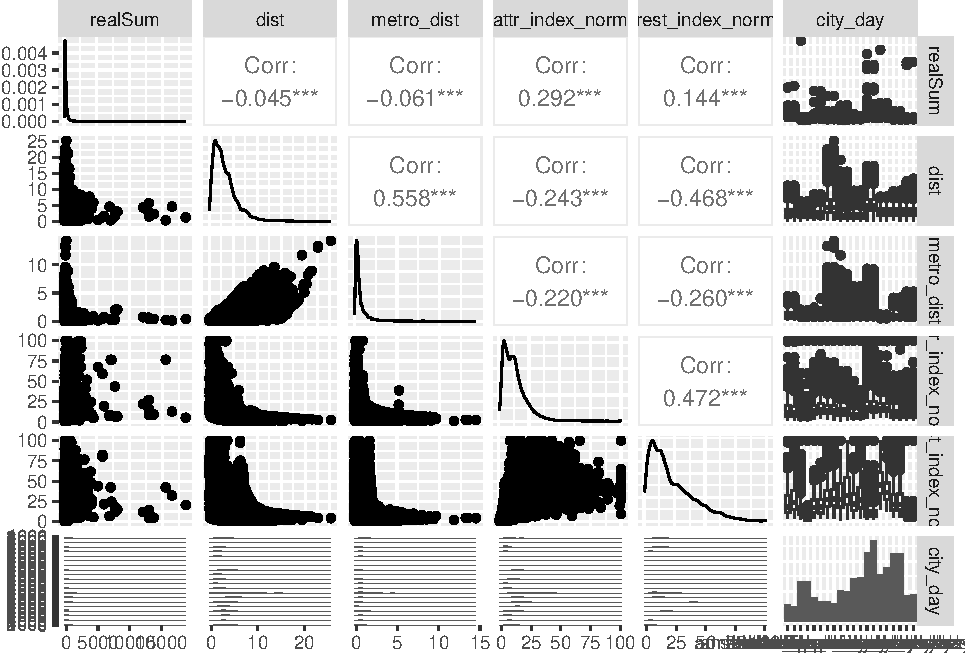
\includegraphics{HW1-Trinath-Sai-Subhash-Reddy-Pittala_files/figure-latex/unnamed-chunk-31-1.pdf}

\begin{Shaded}
\begin{Highlighting}[]
\FunctionTok{ggplot}\NormalTok{(AQSdata, }\FunctionTok{aes}\NormalTok{(}\AttributeTok{x =}\NormalTok{ SITE\_LONGITUDE, }\AttributeTok{y =}\NormalTok{ PM2}\FloatTok{.5}\NormalTok{)) }\SpecialCharTok{+} \FunctionTok{geom\_point}\NormalTok{() }\SpecialCharTok{+}
    \FunctionTok{theme}\NormalTok{(}\AttributeTok{text =} \FunctionTok{element\_text}\NormalTok{(}\AttributeTok{size =} \DecValTok{14}\NormalTok{)) }\SpecialCharTok{+} \FunctionTok{xlab}\NormalTok{(}\StringTok{"Longitude"}\NormalTok{) }\SpecialCharTok{+}
    \FunctionTok{ylab}\NormalTok{(}\StringTok{"PM2.5"}\NormalTok{) }\SpecialCharTok{+} \FunctionTok{coord\_flip}\NormalTok{()}
\end{Highlighting}
\end{Shaded}

\includegraphics{HW1-Trinath-Sai-Subhash-Reddy-Pittala_files/figure-latex/unnamed-chunk-31-2.pdf}

\hypertarget{about-assignment}{%
\section{About Assignment}\label{about-assignment}}

\begin{enumerate}
\def\labelenumi{\arabic{enumi}.}
\setcounter{enumi}{5}
\tightlist
\item
\end{enumerate}

\begin{enumerate}
\def\labelenumi{\alph{enumi}.}
\tightlist
\item
  What is the point of reproducible code?
\end{enumerate}

The point of reproducible code is to make our life easier. Suppose
having a certain set of libraries and formatting types in .rmd file
helps a lot compared to selecting those every single time.

\begin{enumerate}
\def\labelenumi{\alph{enumi}.}
\setcounter{enumi}{1}
\tightlist
\item
  Given an example of why making your code reproducible is important for
  you to know in this class and moving forward.
\end{enumerate}

As explained in former question, reproducibility helps save time by
helping us focus on data rather than worrying about whether a similar
dataset is loaded correctly or not.

\begin{enumerate}
\def\labelenumi{\alph{enumi}.}
\setcounter{enumi}{2}
\tightlist
\item
  On a scale of 1 (easy) -- 10 (hard), how hard was this assignment. If
  this assignment was hard (\textgreater{} 5), please state in one
  sentence what you struggled with.
\end{enumerate}

7

\begin{Shaded}
\begin{Highlighting}[]
\NormalTok{rain.df }\OtherTok{\textless{}{-}} \FunctionTok{mutate}\NormalTok{(rain.df, }\AttributeTok{daily =} \StringTok{\textasciigrave{}}\AttributeTok{0}\StringTok{\textasciigrave{}} \SpecialCharTok{+} \StringTok{\textasciigrave{}}\AttributeTok{1}\StringTok{\textasciigrave{}} \SpecialCharTok{+} \StringTok{\textasciigrave{}}\AttributeTok{2}\StringTok{\textasciigrave{}} \SpecialCharTok{+} \StringTok{\textasciigrave{}}\AttributeTok{3}\StringTok{\textasciigrave{}} \SpecialCharTok{+} \StringTok{\textasciigrave{}}\AttributeTok{4}\StringTok{\textasciigrave{}} \SpecialCharTok{+}
    \StringTok{\textasciigrave{}}\AttributeTok{5}\StringTok{\textasciigrave{}} \SpecialCharTok{+} \StringTok{\textasciigrave{}}\AttributeTok{6}\StringTok{\textasciigrave{}} \SpecialCharTok{+} \StringTok{\textasciigrave{}}\AttributeTok{7}\StringTok{\textasciigrave{}} \SpecialCharTok{+} \StringTok{\textasciigrave{}}\AttributeTok{8}\StringTok{\textasciigrave{}} \SpecialCharTok{+} \StringTok{\textasciigrave{}}\AttributeTok{9}\StringTok{\textasciigrave{}} \SpecialCharTok{+} \StringTok{\textasciigrave{}}\AttributeTok{10}\StringTok{\textasciigrave{}} \SpecialCharTok{+} \StringTok{\textasciigrave{}}\AttributeTok{11}\StringTok{\textasciigrave{}} \SpecialCharTok{+} \StringTok{\textasciigrave{}}\AttributeTok{12}\StringTok{\textasciigrave{}} \SpecialCharTok{+} \StringTok{\textasciigrave{}}\AttributeTok{13}\StringTok{\textasciigrave{}} \SpecialCharTok{+}
    \StringTok{\textasciigrave{}}\AttributeTok{14}\StringTok{\textasciigrave{}} \SpecialCharTok{+} \StringTok{\textasciigrave{}}\AttributeTok{15}\StringTok{\textasciigrave{}} \SpecialCharTok{+} \StringTok{\textasciigrave{}}\AttributeTok{16}\StringTok{\textasciigrave{}} \SpecialCharTok{+} \StringTok{\textasciigrave{}}\AttributeTok{17}\StringTok{\textasciigrave{}} \SpecialCharTok{+} \StringTok{\textasciigrave{}}\AttributeTok{18}\StringTok{\textasciigrave{}} \SpecialCharTok{+} \StringTok{\textasciigrave{}}\AttributeTok{19}\StringTok{\textasciigrave{}} \SpecialCharTok{+} \StringTok{\textasciigrave{}}\AttributeTok{20}\StringTok{\textasciigrave{}} \SpecialCharTok{+} \StringTok{\textasciigrave{}}\AttributeTok{21}\StringTok{\textasciigrave{}} \SpecialCharTok{+} \StringTok{\textasciigrave{}}\AttributeTok{22}\StringTok{\textasciigrave{}} \SpecialCharTok{+}
    \StringTok{\textasciigrave{}}\AttributeTok{23}\StringTok{\textasciigrave{}}\NormalTok{)}
\end{Highlighting}
\end{Shaded}

To find out about how to give numeric column names to a function like
above took me about 1 hour of Googling and Stackoverflow.

\end{document}
